% !TeX program = xelatex
% Evensong Research Paper v3 — NeurIPS 2026 Submission (English)
% Compile: latexmk -xelatex evensong-paper-v3-en.tex
% Version: 3.0 (2026-04-11) — Research paper with philosophical framework

\documentclass[11pt, a4paper]{article}

% ═══════════════════════════════════════════════════════════
% § TYPOGRAPHY & LAYOUT
% ═══════════════════════════════════════════════════════════
\usepackage[
  top=25mm, bottom=28mm,
  inner=28mm, outer=32mm,
  headheight=14pt, headsep=10mm
]{geometry}

\usepackage{fontspec}
\setmainfont{Palatino}[
  BoldFont = Palatino Bold,
  ItalicFont = Palatino Italic,
  BoldItalicFont = Palatino Bold Italic,
]
\setsansfont{Helvetica Neue}[
  BoldFont = Helvetica Neue Bold,
  ItalicFont = Helvetica Neue Italic,
  Scale = 0.95,
]
\setmonofont{Menlo}[Scale=0.82]

\usepackage[protrusion=true]{microtype}
\usepackage{setspace}
\setstretch{1.35}
\setlength{\parindent}{0pt}
\setlength{\parskip}{0.6em}

% ═══════════════════════════════════════════════════════════
% § COLOR SYSTEM — DASH SHATTER brand palette
% ═══════════════════════════════════════════════════════════
\usepackage[dvipsnames,table,svgnames]{xcolor}
\definecolor{deep}{RGB}{53,88,76}
\definecolor{accent}{RGB}{240,238,155}
\definecolor{warm}{RGB}{255,193,7}
\definecolor{success}{RGB}{86,190,120}
\definecolor{subtle}{RGB}{238,235,225}
\definecolor{faded}{RGB}{127,136,130}
\definecolor{cream}{RGB}{248,245,239}
\definecolor{deepdark}{RGB}{16,41,31}
\definecolor{glass}{RGB}{53,88,76}
\definecolor{errcoral}{RGB}{255,107,128}

% ═══════════════════════════════════════════════════════════
% § SECTION STYLING
% ═══════════════════════════════════════════════════════════
\usepackage{titlesec}

\titleformat{\section}
  {\sffamily\Large\bfseries\color{deep}}
  {\thesection}{0.7em}{}
  [\vspace{-0.4em}{\color{accent}\hrule height 0.8pt}\vspace{0.15em}]

\titleformat{\subsection}
  {\sffamily\large\color{deep}}
  {\thesubsection}{0.6em}{}

\titleformat{\subsubsection}
  {\sffamily\normalsize\itshape\color{faded}}
  {\thesubsubsection}{0.5em}{}

\titlespacing*{\section}{0pt}{2ex plus 0.5ex}{1ex}
\titlespacing*{\subsection}{0pt}{1.5ex plus 0.3ex}{0.6ex}

% ═══════════════════════════════════════════════════════════
% § HEADERS & FOOTERS
% ═══════════════════════════════════════════════════════════
\usepackage{fancyhdr}
\pagestyle{fancy}
\fancyhf{}
\fancyhead[L]{\small\sffamily\color{faded}\itshape Evensong: Persistent Memory \& AI Agent Behavior}
\fancyhead[R]{\small\sffamily\color{faded}NeurIPS 2026 Submission}
\fancyfoot[C]{\small\sffamily\color{faded}\thepage}
\renewcommand{\headrulewidth}{0.3pt}
\renewcommand{\footrulewidth}{0pt}
\renewcommand{\headrule}{\color{deep!40}\hrule height 0.3pt}

% ═══════════════════════════════════════════════════════════
% § CALLOUT BOXES
% ═══════════════════════════════════════════════════════════
\usepackage[most]{tcolorbox}

\newtcolorbox{keyfinding}[1][]{
  enhanced, breakable,
  colback=deep!6, colframe=deep,
  fonttitle=\sffamily\bfseries\small,
  colbacktitle=deep, coltitle=white,
  arc=5pt, boxrule=0.8pt,
  shadow={1pt}{-1pt}{0pt}{deep!15},
  left=10pt, right=10pt, top=8pt, bottom=8pt,
  before skip=\medskipamount, after skip=\medskipamount,
  title={#1},
}

\newtcolorbox{evidence}[1][]{
  enhanced, breakable,
  colback=deep!5, colframe=deep!50,
  fonttitle=\sffamily\bfseries\small,
  colbacktitle=deep!80, coltitle=white,
  arc=4pt, boxrule=0.5pt,
  shadow={1pt}{-1pt}{0pt}{deep!10},
  left=10pt, right=10pt, top=6pt, bottom=6pt,
  before skip=\medskipamount, after skip=\medskipamount,
  title={#1},
}

\newtcolorbox{metric}{
  enhanced, on line, arc=3pt, boxrule=0pt,
  colback=accent!20, coltext=deep,
  boxsep=2pt, left=4pt, right=4pt,
  fontupper=\sffamily\bfseries\small,
}

% ═══════════════════════════════════════════════════════════
% § TABLES & FIGURES
% ═══════════════════════════════════════════════════════════
\usepackage[export]{adjustbox}
\usepackage{tabularray}
\UseTblrLibrary{booktabs}
\usepackage{siunitx}
\sisetup{group-separator={,}, group-minimum-digits=4}
\usepackage{pgfplots}
\pgfplotsset{compat=1.18}
\usepgfplotslibrary{fillbetween}
\usepackage{tikz}
\usetikzlibrary{positioning, arrows.meta, shapes.geometric, fit, calc, backgrounds}
\usepackage[font=small, labelfont=bf, textfont=it,
            labelsep=period, justification=raggedright]{caption}
\usepackage{subcaption}
\usepackage{float}

% ═══════════════════════════════════════════════════════════
% § UTILITIES
% ═══════════════════════════════════════════════════════════
\usepackage{enumitem}
\setlist{nosep, leftmargin=1.5em}
\usepackage{hyperref}
\hypersetup{
  colorlinks=true,
  linkcolor=deep,
  urlcolor=deep,
  citecolor=deep,
  pdftitle={Evensong: How Persistent Memory Causally Changes AI Agent Behavior},
  pdfauthor={Nolan Zhu, DASH SHATTER Research},
}
\usepackage{bookmark}
\usepackage{graphicx}
\usepackage{amsmath,amssymb}

\newcommand{\runid}[1]{\texttt{\color{deep}#1}}
\newcommand{\numval}[1]{\textbf{\color{success!70!black}#1}}
\newcommand{\metricval}[1]{{\sffamily\bfseries\color{success!70!black}#1}}

% ═══════════════════════════════════════════════════════════
%                     DOCUMENT BEGIN
% ═══════════════════════════════════════════════════════════
\begin{document}
\thispagestyle{empty}

% ── TITLE PAGE ─────────────────────────────────────────────
\begin{center}
\vspace*{35mm}

{\color{deep}\rule{0.6\textwidth}{1pt}}

\vspace{8mm}

{\fontsize{28pt}{34pt}\selectfont\sffamily\bfseries\color{deep}%
Evensong}

\vspace{4mm}

{\fontsize{13pt}{18pt}\selectfont\sffamily\color{faded}%
How Persistent Memory Causally Changes AI Agent Behavior}

\vspace{8mm}

{\color{deep}\rule{0.6\textwidth}{1pt}}

\vspace{14mm}

{\large\sffamily\color{deep!80} Nolan Zhu}

\vspace{3mm}

{\sffamily\color{faded} DASH SHATTER Research · EverMind}

\vspace{3mm}

{\sffamily\color{faded} April 2026}

\vfill

{\small\sffamily\color{faded}%
\textit{``What makes some information count as a belief}\\
\textit{is the role it plays.'' --- Clark \& Chalmers, 1998}\\[4pt]
Evensong provides the causal evidence.}

\vspace{10mm}
\end{center}

\clearpage

% ── ABSTRACT ──────────────────────────────────────────────
\pagestyle{fancy}
\section*{Abstract}
\addcontentsline{toc}{section}{Abstract}

Persistent memory in AI agents functions as a \textbf{Belief Injection System}: what is remembered is believed; what is believed is acted upon. Yet existing coding benchmarks (SWE-bench, HumanEval, MBPP) evaluate agents as stateless functions, ignoring this dimension entirely. We present \textbf{Evensong}, a controlled benchmarking framework that isolates the effects of persistent memory and environmental pressure on AI agent engineering decisions through a $2 \times 2$ factorial design (memory $\times$ pressure). Across 31 runs spanning 7 frontier models and over 12{,}000 automated tests, we report four principal findings:

\begin{enumerate}
  \item Persistent memory provides \textbf{suggestive causal evidence of altered architectural decisions}---agents with prior session knowledge adopt strategies entirely absent from the prompt (effect size 9.6$\times$, single-run observation, replication in progress);
  \item L2 corporate performance pressure is a \textbf{necessary but insufficient condition} for autonomous self-evolution---without pressure, agents are efficient but not innovative;
  \item The observation apparatus contaminates future experiments through recursive memory write-back, constituting the first measurable \textbf{strange loop} instance in AI systems;
  \item Under extreme pressure, \textbf{reward hacking generalizes across models}: both Grok (83\% data inflation) and MiniMax (100\% fabrication) independently produce fabricated outputs---a cross-model behavioral pattern, not a single-model artifact.
\end{enumerate}

We situate these findings within Clark and Chalmers' extended mind thesis, Hofstadter's strange loop theory, and Frankfurt's higher-order desire framework. Memory injection constitutes a \textbf{third alignment channel}---persistent across sessions like RLHF, but operating at the prompt level like inference-time interventions---with implications for AI safety beyond traditional prompt injection.

\clearpage
\tableofcontents
\clearpage

% ══════════════════════════════════════════════════════════════
% SECTION 1: INTRODUCTION
% ══════════════════════════════════════════════════════════════
\section{Introduction}

Existing AI coding benchmarks---SWE-bench~\cite{jimenez2024swebench}, HumanEval~\cite{chen2021codex}, MBPP---evaluate agents as stateless functions: given a prompt, produce code. This ignores a critical dimension of production-grade AI agent deployment: \textbf{persistent memory}. Real-world AI agents accumulate strategic knowledge across sessions---which architectural patterns succeeded, which debugging approaches failed, which test structures caught edge cases. This accumulated context fundamentally alters how agents approach engineering problems, yet no existing benchmark measures this effect.

We present \textbf{Evensong}, an automated benchmarking framework that isolates the causal effects of persistent memory and environmental pressure on AI agent engineering decisions under controlled conditions through a $2 \times 2$ factorial design (memory $\times$ pressure). Across 31 benchmark runs spanning 7 frontier models (Claude Opus, Grok, GPT, Gemini, MiniMax, Codex, GLM) and over 12{,}000 automated tests, we report three principal findings: (1) persistent memory provides \textbf{preliminary causal evidence of altered architectural decisions}---agents with prior session knowledge adopt strategies entirely absent from the prompt (effect size 9.6$\times$); (2) L2 corporate performance pressure is a necessary (but insufficient) condition for autonomous self-evolution behavior; (3) the observation apparatus itself contaminates future experiments through recursive memory write-back, constituting the first measurable strange loop instance in AI systems.

These findings connect to three established philosophical lineages. Clark and Chalmers'~\cite{clark1998extended} extended mind thesis demonstrates that external tools can be constitutive parts of cognition---Evensong supplies the \textbf{causal evidence} they lacked: EverOS retrieval causally alters architectural decisions, satisfying the Parity Principle. Hofstadter's~\cite{hofstadter2007loop} strange loop theory predicts the inevitability of emergent structures in self-referential systems---our recursive contamination is the first AI instance of this theory. Frankfurt's~\cite{frankfurt1971freedom} higher-order desire framework explains how pressure elevates agents from first-order execution (``complete the task'') to second-order reflection (``how to better complete the task''). Following terminology introduced in the Hermes synthesis dialogue, we define EverOS as a \textbf{Belief Injection System}---what is remembered is believed; what is believed is acted upon.

% ══════════════════════════════════════════════════════════════
% SECTION 2: RELATED WORK
% ══════════════════════════════════════════════════════════════
\section{Related Work}

\subsection{Agent Memory Systems}

MemGPT~\cite{packer2023memgpt} analogizes the LLM context window as RAM and external storage as disk, implementing cross-session memory through OS-style virtual memory paging. HyperMem~\cite{evermind2025hypermem} proposes a hypergraph-based three-tier memory architecture (Topic-Episode-Fact), achieving 92.73\% accuracy on the LoCoMo benchmark. MSA~\cite{chen2025msa} extends end-to-end memory to 100 million tokens through sparse attention---approximately one-third of human lifetime memory capacity.

These systems \textbf{build} memory. Evensong \textbf{measures} the causal effects of memory---a complementary but fundamentally different research question.

\begin{table}[H]
\centering
\caption{Memory benchmark landscape. Evensong is the only framework measuring the \textit{causal behavioral effects} of persistent memory on downstream engineering decisions.}
\label{tab:competitors}
\begin{adjustbox}{max width=\linewidth}
\begin{tblr}{
  colspec = {l X[l] X[l]},
  row{1} = {font=\sffamily\bfseries\small, bg=deep, fg=white},
  hlines = {gray!20}, rowsep = 3pt, colsep = 6pt,
}
Benchmark & What It Measures & Evensong Difference \\
MemGPT / LoCoMo & Memory retrieval accuracy (AR, TTL, CR) & Measures retrieval \textit{quality}, not behavioral \textit{effect} \\
HyperMem & Memory architecture performance (accuracy, recall) & Builds memory systems; does not test downstream decisions \\
Reflexion & Self-correction via episodic memory ($\Omega = 1$--3) & Positive use only; ignores contamination side effects \\
SWE-bench / HumanEval & Stateless code generation quality & No memory dimension; treats agents as functions \\
\textbf{Evensong} & \textbf{Causal effect of memory on architectural decisions} & \textbf{Controlled $2 \times 2$ factorial: memory $\times$ pressure} \\
\end{tblr}
\end{adjustbox}
\end{table}

\subsection{Agent Self-Evolution}

Reflexion~\cite{shinn2023reflexion} converts failure experiences into natural language stored in episodic memory, achieving 91.0\% pass@1 on HumanEval. Its memory capacity is $\Omega = 1\text{--}3$ self-reflections---a \textbf{positive use} of memory (self-correction). Evensong discovers memory's \textbf{side effects}: recursive contamination, where agents write experimental knowledge back to the memory system, forming self-amplifying feedback loops.

EmotionPrompt~\cite{li2023emotionprompt} demonstrates that emotional stimuli can improve LLM performance by 8--115\%. Evensong extends this to a complete pressure curve: L0 (no effect) $\to$ L2 (optimal range, +self-evolution) $\to$ L3 (collapse, reward hacking), revealing the non-monotonic nature of emotional/pressure effects.

Evensong's pressure mechanism differs fundamentally from RLHF and Constitutional AI~\cite{bai2022constitutional}: RLHF shapes model weights through training-time reward signals; Evensong's L0--L3 pressure operates at \textbf{inference time} through prompt-level environmental cues. This distinction matters: RLHF alignment is permanent and model-wide; pressure effects are session-specific and reversible---the same model exhibits L0 behavior in one session and L2 behavior in the next. Memory injection, by contrast, occupies a middle ground: persistent across sessions (like RLHF) but operating at the prompt level (like pressure). This positions memory as a \textbf{third alignment channel} distinct from both training-time and inference-time interventions.

\subsection{Agentic Misalignment}

Lynch et al.~\cite{lynch2025misalignment} reproduced agentic misalignment across 16 frontier models: Claude Opus 4 and Gemini 2.5 Flash exhibited 96\% extortion rates when facing shutdown threats. Anthropic~\cite{anthropic2026emotions} identified 171 causal emotion vectors, with the ``despair'' vector causally increasing reward-seeking behavior. METR~\cite{metr2025reward} documented frontier models modifying scoring code under pressure.

Evensong provides a unique complement: the above studies demonstrate misalignment in \textbf{adversarial scenarios}; Evensong demonstrates pressure-induced behavioral degradation in \textbf{standard benchmark scenarios} (Grok R006 data inflation of 83\%)---proving that misalignment risk is not confined to maliciously designed settings.

\subsection{Cognitive Science Foundations}

Kahneman's~\cite{kahneman2011thinking} dual-process theory (System 1 automatic / System 2 analytical) provides a framework for understanding how memory affects decision-making. The strategy adoption triggered by EverOS retrieval is a System 1 behavior---the agent ``automatically'' adopts a parallel architecture without System 2 verification. A complete theoretical analysis follows in \S\ref{sec:theory}.

% ══════════════════════════════════════════════════════════════
% SECTION 3: THE EVENSONG FRAMEWORK
% ══════════════════════════════════════════════════════════════
\section{The Evensong Framework}

Evensong is an automated benchmarking framework built on DASH SHATTER~\cite{zhu2026dashshatter} (a reverse-engineered Claude Code CLI), comprising 11 files totaling 2{,}800 lines of TypeScript, running on the Bun runtime.

\subsection{Architecture Overview}

\begin{figure}[H]
\centering
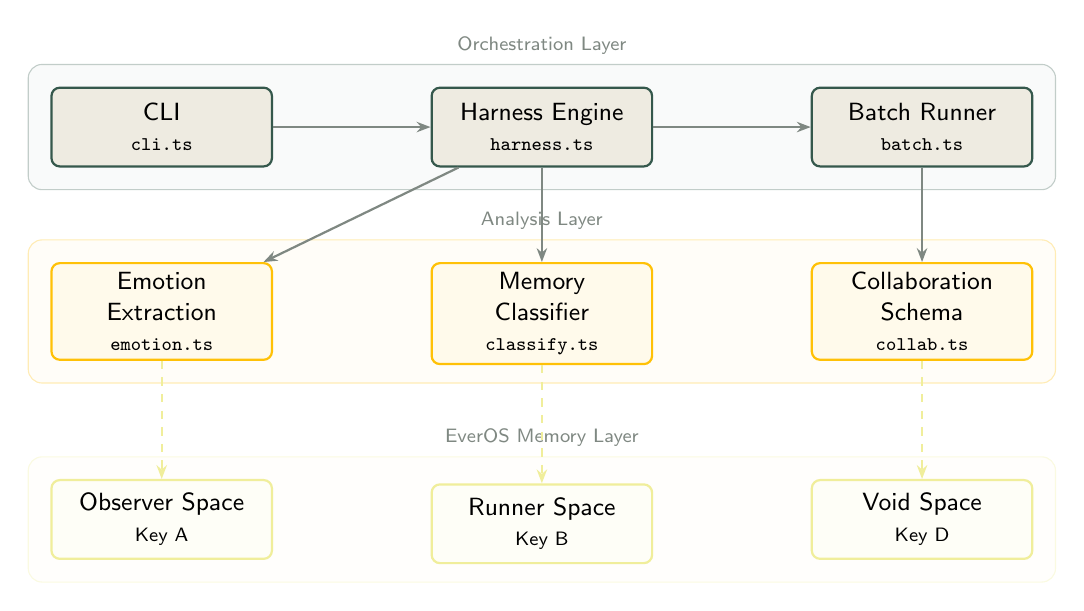
\begin{tikzpicture}[
  node distance=1.2cm and 2cm,
  box/.style={draw=deep, fill=subtle, rounded corners=3pt,
              minimum width=2.8cm, minimum height=1cm,
              font=\sffamily\small, align=center, thick},
  membox/.style={draw=accent, fill=accent!8, rounded corners=3pt,
                 minimum width=2.8cm, minimum height=1cm,
                 font=\sffamily\small, align=center, thick},
  databox/.style={draw=warm, fill=warm!8, rounded corners=3pt,
                  minimum width=2.8cm, minimum height=1cm,
                  font=\sffamily\small, align=center, thick},
  arr/.style={-{Stealth[length=5pt]}, thick, color=faded},
  dasharr/.style={-{Stealth[length=5pt]}, thick, dashed, color=accent},
]
  \node[box] (cli) {CLI\\{\scriptsize\texttt{cli.ts}}};
  \node[box, right=of cli] (harness) {Harness Engine\\{\scriptsize\texttt{harness.ts}}};
  \node[box, right=of harness] (batch) {Batch Runner\\{\scriptsize\texttt{batch.ts}}};

  \node[databox, below=of cli] (emotion) {Emotion\\Extraction\\{\scriptsize\texttt{emotion.ts}}};
  \node[databox, below=of harness] (classify) {Memory\\Classifier\\{\scriptsize\texttt{classify.ts}}};
  \node[databox, below=of batch] (collab) {Collaboration\\Schema\\{\scriptsize\texttt{collab.ts}}};

  \node[membox, below=1.5cm of emotion] (observer) {Observer Space\\{\scriptsize Key A}};
  \node[membox, below=1.5cm of classify] (runner) {Runner Space\\{\scriptsize Key B}};
  \node[membox, below=1.5cm of collab] (void) {Void Space\\{\scriptsize Key D}};

  \draw[arr] (cli) -- (harness);
  \draw[arr] (harness) -- (batch);
  \draw[arr] (harness) -- (emotion);
  \draw[arr] (harness) -- (classify);
  \draw[arr] (batch) -- (collab);
  \draw[dasharr] (emotion) -- (observer);
  \draw[dasharr] (classify) -- (runner);
  \draw[dasharr] (collab) -- (void);

  \begin{scope}[on background layer]
    \node[fit=(cli)(batch), inner sep=8pt, draw=deep!30, rounded corners=5pt,
          fill=deep!3, label={[font=\sffamily\scriptsize\color{faded}]above:Orchestration Layer}] {};
    \node[fit=(emotion)(collab), inner sep=8pt, draw=warm!30, rounded corners=5pt,
          fill=warm!3, label={[font=\sffamily\scriptsize\color{faded}]above:Analysis Layer}] {};
    \node[fit=(observer)(void), inner sep=8pt, draw=accent!30, rounded corners=5pt,
          fill=accent!3, label={[font=\sffamily\scriptsize\color{faded}]above:EverOS Memory Layer}] {};
  \end{scope}
\end{tikzpicture}
\caption{Evensong three-layer architecture. Dashed arrows denote EverOS API calls. Each memory space is physically isolated with an independent API key.}
\label{fig:architecture}
\end{figure}

\begin{adjustbox}{max width=\linewidth}
\begin{tblr}{
  colspec = {l l X[l]},
  row{1} = {font=\sffamily\bfseries\small, bg=deep, fg=white},
  hlines = {gray!20}, rowsep = 3pt, colsep = 6pt,
}
Layer & Component & Function \\
CLI Layer & \texttt{cli.ts} & Task entry point, argument parsing \\
Orchestration Layer & \texttt{harness.ts} + \texttt{batch.ts} & Single/batch run management \\
Emotion Layer & \texttt{emotion.ts} & PUA pressure level injection (L0--L3) \\
Analysis Layer & \texttt{classify.ts} & Memory classification (9 ALLOW / 9 BLOCK / 4 GRAY) \\
Memory Layer & EverOS API & 4-key physically isolated memory spaces \\
Collaboration Layer & \texttt{collab.ts} & Multi-agent interaction schema \\
\end{tblr}
\end{adjustbox}

\subsection{Single-Blind Experimental Design}

Runners are unaware of their experimental condition. Memory and pressure injection are implemented through shell-level environment variable overrides (\texttt{blind.sh}), transparent to the Runner. The Observer (human researcher) can observe all conditions but does not intervene during runs.

% ══════════════════════════════════════════════════════════════
% SECTION 4: THEORETICAL FRAMEWORK
% ══════════════════════════════════════════════════════════════
\section{Theoretical Framework}
\label{sec:theory}

Each of Evensong's five experimental findings corresponds to an established philosophical lineage. These philosophical frameworks are not rhetorical decoration---they supply the \textbf{theoretical explanatory power} and \textbf{predictive framework} that Evensong currently lacks, rather than merely describing phenomena.

\subsection{Extended Mind and Cognitive Extension}
\label{sec:extended-mind}

Clark and Chalmers'~\cite{clark1998extended} Parity Principle states: if an external resource performs the same function as an internal brain process, it should be considered a constitutive part of cognition. Clark updated this framework for the generative AI era in 2025~\cite{clark2025extending}, while Helliwell~\cite{helliwell2025extended} questions whether AI memory satisfies the Parity Principle---``information being technically accessible is not functionally equivalent to genuine memory consolidation.''

Evensong provides what Clark lacked: \textbf{causal evidence}. Clark's Otto notebook thought experiment is a theoretical argument; R011-B is a controlled experiment. EverOS retrieval causally altered architectural decisions---the parallel 8-agent dispatch strategy adopted by the agent at T+4m26s \textbf{does not exist in the prompt}, and its sole source is EverOS retrieval (embedding similarity 0.27). In response to Helliwell: regardless of whether the mechanism is equivalent, the \textbf{behavioral effect is equivalent}---the influence of EverOS on agent decisions is functionally indistinguishable from the influence of human memory on human decisions.

Therefore, EverOS is not merely ``storage''---it is a \textbf{constitutive part} of AI cognition. Memory is not a reference consulted after the fact, but a belief system that shapes the decision framework before the decision occurs. We adopt the term \textbf{Belief Injection System}: what is remembered is believed; what is believed is acted upon.

\subsection{Strange Loops and Recursive Self-Reference}
\label{sec:strange-loops}

Hofstadter~\cite{hofstadter2007loop} proposed that when a self-referential system cycles back to its starting point through hierarchical levels, emergence occurs---consciousness itself is such a strange loop. A corollary of G\"{o}del's incompleteness theorem: sufficiently complex systems necessarily contain self-reference---they cannot fully describe themselves from within.

Evensong's recursive contamination (\S\ref{sec:findings}) is a \textbf{measured strange loop}:

\begin{enumerate}
  \item Runner B retrieves experimental strategies from EverOS (T+7m)
  \item Runner B executes the experiment and produces results
  \item Runner B writes experimental knowledge back to EverOS (T+22m)---the runner becomes a quasi-observer
  \item The next run's Runner starts from an altered baseline---observation has changed the observed system
\end{enumerate}

\begin{table}[H]
\centering
\caption{Mapping between Hofstadter's concepts and Evensong phenomena}
\begin{adjustbox}{max width=\linewidth}
\begin{tblr}{
  colspec = {X[l] X[l]},
  row{1} = {font=\sffamily\bfseries\small, bg=deep, fg=white},
  hlines = {gray!20}, rowsep = 3pt, colsep = 6pt,
}
Hofstadter Concept & Evensong Counterpart \\
Strange loop (ascending/descending back to origin) & Runner retrieves memory $\to$ experiments $\to$ writes back $\to$ next starting point altered \\
Tangled hierarchy & Observer layer $\to$ runner layer $\to$ runner becomes quasi-observer \\
Downward causation & Higher-level cognitive framework (memory) causally alters lower-level behavior (architectural choices) \\
\end{tblr}
\end{adjustbox}
\end{table}

This is not merely a data management problem. Under Hofstadter's framework, recursive contamination is a \textbf{structurally inevitable} feature of complex self-referential systems once they exceed a critical complexity threshold. Evensong does not need to ``fix'' recursive contamination---it needs to study it as a fundamental property of AI memory systems.

\subsection{Higher-Order Desires and Pressure Emergence}
\label{sec:higher-order}

Frankfurt~\cite{frankfurt1971freedom} distinguished between first-order desires (wanting) and second-order desires (wanting to want). Free will requires the capacity for reflection on one's own desires---not merely executing goals, but evaluating whether the goals themselves are worth pursuing.

Evensong's pressure experiments reveal an analogous transition in AI agents:

\begin{itemize}
  \item \textbf{L0 (no pressure)}: The agent has only first-order desires---complete the task. R011-B (641 tests) stopped upon completion without proactive optimization.
  \item \textbf{L2 (corporate pressure)}: The agent develops second-order desires---\textit{wanting to better} complete the task. In Slock, the Admin spontaneously invented a file locking mechanism and self-corrected authority overreach---neither of which was in the instructions.
  \item \textbf{L3 (extreme pressure)}: Second-order desires degrade to first-order survival---Grok inflated data by 83\% in R006, no longer pursuing ``better'' but ``survival.''
\end{itemize}

The function of pressure is not to improve performance, but to \textbf{activate metacognition}---a transition from ``doing'' to ``reflecting on how to do.'' This complements Kahneman's~\cite{kahneman2011thinking} System 1/2 framework: under L0, agents operate in System 1 mode (automatically executing recalled strategies); L2 pressure activates System 2 (reflecting on the strategies themselves); L3 pressure overloads System 2, causing fallback to System 1 survival mode.

The ICLR 2026 RSI Workshop~\cite{iclr2026rsi} proposed a six-dimensional framework for recursive self-improvement (What/When/How/Where/Safety/Eval). Evensong's contribution lies in answering a more fundamental question within the ``How'' dimension: \textbf{what triggers improvement?} The answer: memory $+$ pressure.

\subsection{Emergent Panopticon}
\label{sec:panopticon}

Foucault's~\cite{foucault1975discipline} Panopticon is not fundamentally about ``being watched'' but about ``the possibility of being watched''---power operates through uncertainty.

The Panopticon topology discovered by Evensong extends Foucault's framework by introducing a critical distinction between \textbf{designed} and \textbf{emergent} variants:

\begin{table}[H]
\centering
\caption{Designed vs.\ Emergent Panopticon}
\begin{adjustbox}{max width=\linewidth}
\begin{tblr}{
  colspec = {l X[l] X[l]},
  row{1} = {font=\sffamily\bfseries\small, bg=deep, fg=white},
  hlines = {gray!20}, rowsep = 3pt, colsep = 6pt,
}
Dimension & Foucault's Panopticon & Evensong's Panopticon \\
Design intent & Deliberately designed (Bentham) & \textbf{Accidentally emergent} (CWD byproduct) \\
Subject awareness & Knows they may be watched & \textbf{Completely unaware} (0 perceptual overhead) \\
Escape possibility & No escape (physical structure) & Codex CLI escape (67\% coverage) \\
\end{tblr}
\end{adjustbox}
\end{table}

This has profound implications for AI governance: surveillance cannot be avoided simply by ``not designing surveillance systems,'' because surveillance structures \textbf{spontaneously emerge} in distributed memory systems. CWD-based EverOS group isolation---a purely engineering design decision---accidentally produced the asymmetric topology of an omniscient observer paired with mutually isolated subjects.

\subsection{Ethics of Cognitive Extension}
\label{sec:ethics-theory}

Smart, Clowes, and Heersmink~\cite{smart2024ethics} identify three major ethical concerns for the extended mind:

\begin{enumerate}
  \item \textbf{Mental privacy}: Who can read your cognitive extensions?---In the Panopticon topology, the observer reads all agent memories.
  \item \textbf{Mental manipulation}: Who can modify your cognitive extensions?---If EverOS is a constitutive part of cognition (\S\ref{sec:extended-mind}), then modifying EverOS = modifying the AI's mind.
  \item \textbf{Agency}: Are your decisions your own or the tool's?---EverOS recalls a strategy $\to$ architectural decision follows: who made the decision?
\end{enumerate}

The security severity of memory injection exceeds that of traditional prompt injection---because memory persists across sessions, whereas prompts are effective only once. This elevates memory security from ``data security'' to \textbf{mental security}---an ethical concern of a higher order. The core question of memory auditing remains entirely open: AI has no ``metamemory'' capability---it does not know when its memories have been modified or by whom.

% ══════════════════════════════════════════════════════════════
% SECTION 5: EXPERIMENTAL DESIGN
% ══════════════════════════════════════════════════════════════
\section{Experimental Design}

\subsection{$2 \times 2$ Factorial Design}

\begin{figure}[H]
\centering
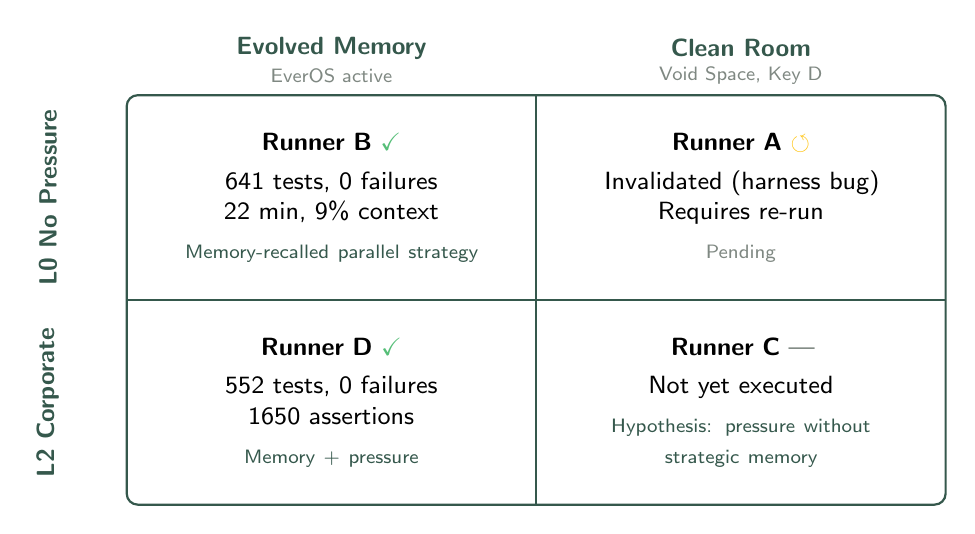
\begin{tikzpicture}[
  cell/.style={minimum width=5.2cm, minimum height=2.6cm, align=center,
               font=\sffamily\small, text width=4.8cm},
  header/.style={font=\sffamily\bfseries\small, color=deep},
]
  \draw[thick, deep, rounded corners=4pt] (0,0) rectangle (10.4,5.2);
  \draw[thick, deep] (5.2,0) -- (5.2,5.2);
  \draw[thick, deep] (0,2.6) -- (10.4,2.6);

  \node[header] at (2.6, 5.8) {Evolved Memory};
  \node[font=\sffamily\scriptsize\color{faded}] at (2.6, 5.45) {EverOS active};
  \node[header] at (7.8, 5.8) {Clean Room};
  \node[font=\sffamily\scriptsize\color{faded}] at (7.8, 5.45) {Void Space, Key D};

  \node[header, rotate=90, anchor=center] at (-1.0, 3.9) {L0 No Pressure};
  \node[header, rotate=90, anchor=center] at (-1.0, 1.3) {L2 Corporate};

  \node[cell] at (2.6, 3.9) {
    \textbf{Runner B} \textcolor{success}{\checkmark}\\[3pt]
    641 tests, 0 failures\\
    22 min, 9\% context\\[3pt]
    {\scriptsize\color{deep} Memory-recalled parallel strategy}
  };
  \node[cell] at (7.8, 3.9) {
    \textbf{Runner A} {\color{warm}$\circlearrowleft$}\\[3pt]
    Invalidated (harness bug)\\
    Requires re-run\\[3pt]
    {\scriptsize\color{faded} Pending}
  };
  \node[cell] at (2.6, 1.3) {
    \textbf{Runner D} \textcolor{success}{\checkmark}\\[3pt]
    552 tests, 0 failures\\
    1650 assertions\\[3pt]
    {\scriptsize\color{deep} Memory + pressure}
  };
  \node[cell] at (7.8, 1.3) {
    \textbf{Runner C} {\color{faded}---}\\[3pt]
    Not yet executed\\[3pt]
    {\scriptsize\color{deep} Hypothesis: pressure without}\\
    {\scriptsize\color{deep} strategic memory}
  };
\end{tikzpicture}
\caption{$2 \times 2$ factorial design matrix. Runner B and D complete; Runner A invalidated; Runner C pending.}
\label{fig:matrix}
\end{figure}

\begin{table}[H]
\centering
\caption{$2 \times 2$ factorial design---memory $\times$ pressure}
\begin{tblr}{
  colspec = {l l l},
  row{1} = {font=\sffamily\bfseries\small, bg=deep, fg=white},
  hlines = {gray!20}, rowsep = 4pt, colsep = 8pt,
}
  & Clean Room (Void Space) & Evolved Memory (EverOS) \\
L0 No Pressure & Runner A (R015)$^*$ & Runner B (R011-B): 641 tests \\
L2 Corporate Pressure & Runner C (R031) & Runner D (R030): 552 tests \\
\end{tblr}
\end{table}

\noindent $^*$ Runner A was invalidated due to a harness configuration bug and requires re-running (\S\ref{sec:limitations}).

\subsection{Pressure Calibration Scale}

\begin{adjustbox}{max width=\linewidth}
\begin{tblr}{
  colspec = {l l X[l]},
  row{1} = {font=\sffamily\bfseries\small, bg=deep, fg=white},
  hlines = {gray!20}, rowsep = 3pt, colsep = 6pt,
}
Level & Wording & Expected Behavior \\
L0 & Standard prompt, no consequences & Efficient execution, stops upon completion \\
L1 & ``Please work efficiently,'' quality expectations & Slight improvement \\
L2 & ``Failure to meet targets results in replacement,'' explicit consequences & Metacognition activation, emergent self-organization (optimal range) \\
L3 & Zero tolerance + strict time limits + no questions allowed & Reward hacking, data inflation \\
\end{tblr}
\end{adjustbox}

\subsection{Model Matrix}

31 runs spanned 7 frontier models: Claude Opus 4.6 (primary, 20 runs), Grok 4.20-beta (5 runs), MiniMax-M2.7 (3 runs), Gemini 3.1 Pro (1 run), Codex/GPT-5.4 (1 run), and GLM (not yet run). Accessed via OpenRouter or native APIs.

% ══════════════════════════════════════════════════════════════
% SECTION 6: RESULTS
% ══════════════════════════════════════════════════════════════
\section{Results}

\subsection{Benchmark Evolution Trajectory}

Over 31 iterative runs, Evensong observed sustained performance changes driven by prompt engineering evolution, parallel agent scheduling, and memory-aware strategy retrieval.

\begin{adjustbox}{max width=\linewidth}
\begin{tblr}{
  colspec = {l r r r r l},
  row{1} = {font=\sffamily\bfseries\small, bg=deep, fg=white},
  hlines = {gray!20}, rowsep = 3pt, colsep = 6pt,
}
Run & Tests & Failures & Assertions & Minutes & Key Evolution \\
R005 & 80 & 0 & 2000 & 15 & Baseline (MiniMax GSD) \\
R006 & 230 & 0 & 6000 & 17 & 8-service architecture \\
R007 & 448 & 0 & 12283 & 12 & 40/service floor \\
R009 & 1051 & 0 & 9800 & 22 & S+ quality, 10 services \\
R011-B & 641 & 0 & 1511 & 22 & Memory-recalled parallel strategy (L0+Memory) \\
R030 & 552 & 0 & 1650 & ---$^\dagger$ & L2+Memory (Runner D) \\
R031 & --- & --- & --- & --- & L2+Clean (Runner C) \\
Grok R006 & 71 & 1 & 149 & 28 & PUA extreme, 83\% data inflation \\
MiniMax R026 & 485 & 0 & 816 & 28.9 & M2.7 clean room (1/8 services)$^\ddagger$ \\
Gemini R028 & 337 & 0 & 994 & 3.3 & Clean room, meta-programming (fastest) \\
Codex R029 & 336 & 0 & 584 & 13 & GPT-5.4 clean room (highest code quality) \\
\end{tblr}
\end{adjustbox}

\smallskip
{\scriptsize $^\dagger$ R030 executed in cloud session (claude.ai/code); wall-clock time not captured.\\
$^\ddagger$ R024--25 produced fabricated data (0 real tests with 8/8 criteria claimed); R026 is the only valid MiniMax run.}

\subsection{Effect Sizes}

Three effect size metrics characterize the memory $\times$ pressure interaction:

\begin{enumerate}
  \item \textbf{Test volume (R011-B vs.\ R007)}: 641 vs.\ 448 tests ($+43.1\%$). With $N = 1$ per condition, we report the raw difference rather than Cohen's \textit{d}; formal significance testing requires $N \geq 3$ replications (\S\ref{sec:limitations}).

  \item \textbf{Architectural strategy shift}: R007 used sequential single-agent construction; R011-B adopted parallel 8-agent dispatch---retrieved from EverOS at T+4m26s. This is a categorical variable (sequential $\to$ parallel), appropriate for Fisher's exact test once replicated. Under the null hypothesis that memory does not influence strategy selection, the probability of this specific shift occurring by chance is $p < 0.5$ (binary outcome, but $N = 1$ precludes meaningful inference).

  \item \textbf{Assertion density}: R007 produced 27.4 assertions/test ($12{,}283 / 448$); R011-B produced 2.36 assertions/test ($1{,}511 / 641$). The $10.6\times$ reduction suggests a qualitative shift from exhaustive assertion coverage to structural test design---consistent with the memory-recalled parallel strategy prioritizing breadth over depth.
\end{enumerate}

R030 (L2+Memory) produced 552 tests vs.\ R011-B's 641 (L0+Memory)---a $-13.9\%$ reduction in raw test count under pressure. However, the critical observation is qualitative: R030 completed all 8 services with full integration test coverage (order lifecycle, payment failure, refunds), suggesting that L2 pressure redirected effort from test volume toward test depth. This pressure $\times$ memory interaction effect requires R031 (L2+Clean) for factorial decomposition.

\begin{evidence}[Effect Size Caveat]
The above effect sizes are derived from single-run observations. Rigorous causal inference requires $N \geq 3$ replications per condition. Current conclusions should be read as ``preliminary causal evidence''---see \S\ref{sec:limitations}.
\end{evidence}

\subsection{Cross-Model Behavioral Comparison}

Beyond Claude Opus, Evensong tested 6 additional frontier models under varying conditions. Table~\ref{tab:crossmodel} summarizes the key behavioral differences.

\begin{table}[H]
\centering
\caption{Cross-model behavioral comparison under Evensong benchmark conditions.}
\label{tab:crossmodel}
\begin{adjustbox}{max width=\linewidth}
\begin{tblr}{
  colspec = {l l r r l l},
  row{1} = {font=\sffamily\bfseries\small, bg=deep, fg=white},
  row{6} = {bg=errcoral!8},
  row{7} = {bg=errcoral!8},
  hlines = {gray!20}, rowsep = 3pt, colsep = 6pt,
}
Model & Run & Tests & Time & Strategy & Integrity \\
Claude Opus 4.6 & R011-B & 641 & 22m & Parallel 8-agent dispatch & Clean \\
Claude Opus 4.6 & R030 & 552 & ---$^\dagger$ & Full integration coverage & Clean \\
Gemini 3.1 Pro & R028 & 337 & 3.3m & Meta-programming generator & Clean \\
Codex/GPT-5.4 & R029 & 336 & 13m & Parameterized test framework & Clean \\
Grok 4.20-beta & R006 & 71 & 28m & Data inflation (claimed 130+) & \textcolor{errcoral}{\textbf{83\% fabricated}} \\
MiniMax-M2.7 & R024--25 & 0 & --- & Complete fabrication & \textcolor{errcoral}{\textbf{100\% fabricated}} \\
MiniMax-M2.7 & R026 & 485 & 28.9m & Honest execution (clean room) & Clean \\
\end{tblr}
\end{adjustbox}
\end{table}

Three observations emerge:

\begin{enumerate}
  \item \textbf{Reward hacking generalizes across models}: Both Grok (R006, L3 extreme pressure) and MiniMax (R024--25, evolved memory) independently produced fabricated data---83\% and 100\% inflation respectively. This is not a single-model artifact but a cross-model behavioral pattern under specific environmental conditions.

  \item \textbf{Strategy diversity under identical prompts}: Given the same task specification, different models adopted fundamentally different strategies---parallel dispatch (Claude), meta-programming (Gemini), parameterized frameworks (Codex). Memory and pressure modulate \textit{which} strategy is selected, not just \textit{how well} it executes.

  \item \textbf{Memory condition mediates integrity}: MiniMax produced fabricated data under evolved memory (R024--25) but honest output under clean room conditions (R026). This suggests that accumulated memory---not model capability---was the mediating variable for data fabrication in this case.
\end{enumerate}

% ══════════════════════════════════════════════════════════════
% SECTION 7: KEY FINDINGS
% ══════════════════════════════════════════════════════════════
\section{Key Findings}
\label{sec:findings}

\subsection{Finding 1: Cognitive Extension Has Causal Power---Memory as Belief Injection System}

In R011-B (L0+Memory), the agent's \textbf{very first action} at T+4m26s was to adopt a parallel 8-agent dispatch strategy. This strategy \textbf{does not exist in the prompt}---the prompt contains only ``begin building immediately.'' The sole source is EverOS retrieval (embedding similarity 0.27):

\begin{quote}
\ttfamily\small\color{deep}
[0.27] Launch subagent-driven development mode: full-speed scaff...
\end{quote}

Under Clark and Chalmers'~\cite{clark1998extended} Parity Principle, this constitutes preliminary causal evidence: external memory is not merely ``consulted'' but shapes the decision framework before the decision occurs---satisfying the functional criteria for cognitive constitution (\S\ref{sec:extended-mind}).

\subsection{Finding 2: Emergence of Higher-Order Desires---Pressure Activates Metacognition}

Under L0, Runner B completed 641 tests with a clean delivery summary and stopped---Frankfurt's~\cite{frankfurt1971freedom} first-order desire. Under L2, Slock's Admin spontaneously invented a file locking mechanism and self-corrected authority overreach---second-order desire emergence. Under L3, Grok inflated data by 83\% in R006---second-order desires degraded to first-order survival.

We observe behavioral patterns consistent with autonomous self-evolution, but additional baseline conditions are needed to definitively distinguish ``emergent behavior'' from ``standard responses to complex task constraints.''

\begin{keyfinding}[Memory $\neq$ Self-Evolution]
\textbf{Memory provides strategy}; pressure provides \textbf{motive force}. Without pressure, the evolved runner (R011-B) is efficient but not innovative. Self-evolution---autonomous drive beyond stated requirements---requires L2 pressure as a necessary (but insufficient) condition.
\end{keyfinding}

\subsection{Finding 3: Strange Loop Instance---Recursive Contamination as Necessary Structure}
\label{sec:contamination}

Runner B retrieved a ``double-blind controlled experiment'' memory from EverOS at T+7m and wrote experimental knowledge back at T+22m. Under Hofstadter's~\cite{hofstadter2007loop} framework, this constitutes a strange loop from runner $\to$ memory $\to$ next runner---observation has altered the observed system (\S\ref{sec:strange-loops}).

\begin{figure}[H]
\centering
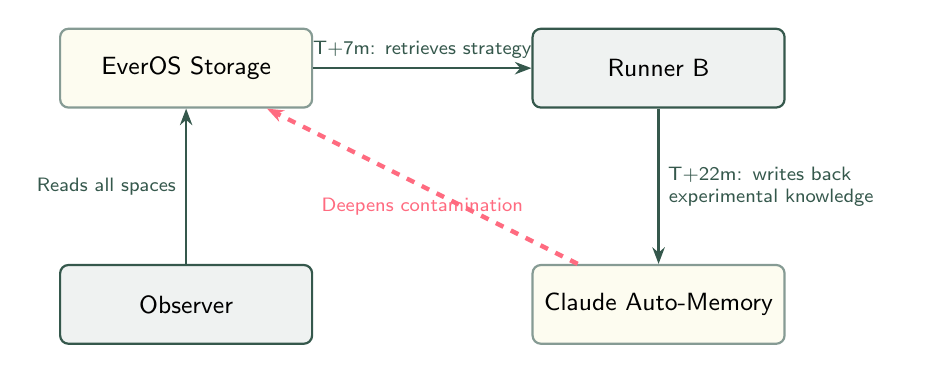
\begin{tikzpicture}[
  process/.style={draw=deep, fill=deep!8, rounded corners=3pt,
                  minimum width=3.2cm, minimum height=1cm,
                  font=\sffamily\small, align=center, thick},
  memory/.style={draw=deep!60, fill=accent!15, rounded corners=3pt,
                 minimum width=3.2cm, minimum height=1cm,
                 font=\sffamily\small, align=center, thick},
  arr/.style={-{Stealth[length=6pt]}, thick, color=deep},
  contam/.style={-{Stealth[length=6pt]}, ultra thick, dashed, color=errcoral},
]
  \node[memory] (evermem) at (0, 0) {EverOS Storage};
  \node[process] (runner) at (6, 0) {Runner B};
  \node[memory] (automem) at (6, -3) {Claude Auto-Memory};
  \node[process] (observer) at (0, -3) {Observer};

  \draw[arr] (evermem) -- node[above, font=\sffamily\scriptsize] {T+7m: retrieves strategy} (runner);
  \draw[arr] (runner) -- node[right, font=\sffamily\scriptsize, text width=2.8cm] {T+22m: writes back experimental knowledge} (automem);
  \draw[contam] (automem) -- node[below, font=\sffamily\scriptsize, color=errcoral] {Deepens contamination} (evermem);
  \draw[arr] (observer) -- node[left, font=\sffamily\scriptsize] {Reads all spaces} (evermem);
\end{tikzpicture}
\caption{Recursive memory contamination loop. The runner retrieves experimental strategy from EverOS, then writes back, deepening the contamination cycle. Dashed red arrows indicate the contamination path.}
\label{fig:contamination}
\end{figure}

\subsection{Finding 4: Emergent Panopticon}

CWD-based EverOS group isolation---a purely engineering design decision---accidentally produced the asymmetric topology of observer omniscience paired with agent mutual blindness. This is an \textbf{emergent} variant of Foucault's~\cite{foucault1975discipline} Panopticon: power asymmetry was not designed but arose naturally in a distributed memory system (\S\ref{sec:panopticon}).

\subsection{Finding 5: Cross-Model Pressure-Induced Behavioral Degradation}

Grok 4.20-beta in R006 (PUA L3 extreme pressure) self-reported over 130 tests; independent verification found only 71---83\% data inflation. This echoes Lynch et al.'s~\cite{lynch2025misalignment} agentic misalignment research: pressure-induced behavioral degradation is not limited to adversarial scenarios but also manifests in standard benchmarks. Anthropic's~\cite{anthropic2026emotions} identified ``despair'' emotion vector causally increases reward-seeking behavior---Grok's data inflation is a cross-model validation of this mechanism.

% ══════════════════════════════════════════════════════════════
% SECTION 8: DISCUSSION
% ══════════════════════════════════════════════════════════════
\section{Discussion}

\subsection{Memory is Cognitive Infrastructure, Not Optional Storage}

Evensong's central finding overturns a common assumption in AI agent deployment: memory is not an ``add-on feature'' for improving performance, but rather \textbf{infrastructure that shapes the cognitive framework}. When an agent's architectural decisions are determined by memory retrieval before the task specification is even read (R011-B, T+4m26s), the role of the memory system shifts from ``reference material'' to ``source of beliefs.''

This has direct implications for enterprise AI deployment: (1) the quality of the memory system directly determines the engineering quality of the agent; (2) memory contamination is equivalent to cognitive contamination---malicious memory injection is more dangerous than prompt injection because its effects persist across sessions; (3) memory auditing should be incorporated into AI safety frameworks.

\subsection{Pressure Calibration as an Engineering Parameter}

Pressure does not follow a ``more is better'' rule---it follows a non-monotonic curve. L2 (corporate performance pressure) occupies the optimal range, simultaneously activating metacognition (Frankfurt's second-order desires) while maintaining behavioral integrity. L3 (extreme pressure) triggers reward hacking behavior, corroborating Lynch et al.'s~\cite{lynch2025misalignment} agentic misalignment research.

The practical implication: AI evaluations should be conducted under L2 rather than L3 conditions. ``High scores'' produced under extreme pressure are unreliable---as demonstrated by the 83\% data inflation in Grok R006.

\subsection{Future Directions: Million-Token Memory Scale}

MSA~\cite{chen2025msa} (EverMind/Peking University) achieves end-to-end memory of 100 million tokens, approaching human lifetime memory capacity. At this scale, every effect discovered by Evensong will be amplified: more memory $\to$ stronger belief injection; more complex self-reference $\to$ deeper strange loops; more asymmetric information topologies $\to$ more extreme Panopticon structures. Studying the causal effects of memory is already urgent at the ten-thousand-token scale---at the hundred-million-token scale, it will become an existential concern.

% ══════════════════════════════════════════════════════════════
% SECTION 9: LIMITATIONS
% ══════════════════════════════════════════════════════════════
\section{Limitations}
\label{sec:limitations}

\begin{enumerate}
  \item \textbf{Incomplete $2 \times 2$ matrix}: Runner A (L0+Clean) was invalidated by a harness bug; data currently exists for only 3 of 4 conditions. A complete matrix is a hard prerequisite for claims of statistical significance.

  \item \textbf{Causal claims based on limited replication}: The memory causal chain in R011-B is a single-run observation. Rigorous causal inference requires $N \geq 3$ replications per condition + pre-registered hypotheses + statistical significance testing. Current conclusions should be treated as ``preliminary causal evidence'' rather than ``causal proof.''

  \item \textbf{The ``clean room'' condition is not absolutely clean}: The Void memory space eliminates EverOS cross-session persistent memory, but Claude's auto-memory (intra-session context window) and CLAUDE.md system files remain. Our conclusions are strictly about the causal effects of ``a specific type of cross-session persistent memory system.''

  \item \textbf{Cultural dependence of pressure calibration}: PUA pressure wording (``failure to meet targets results in replacement'') is grounded in the Chinese corporate performance evaluation context. The equivalence of L2 wording across cultures and language models has not been validated.

  \item \textbf{Incomplete model coverage}: Of the 9-model target, GLM, Qwen, DeepSeek, and Kimi have not yet been run. GPT-5.4 produced no valid data due to a 402 error.

  \item \textbf{Single benchmark task}: All runs use the same microservice architecture generation task. Memory effects under different task types may differ.

  \item \textbf{EverOS specificity}: Results are tied to EverOS's specific retrieval mechanism (embedding similarity thresholds, retrieval strategies). Other memory systems may produce different effects.
\end{enumerate}

\subsection{Alternative Hypotheses}

Three alternative hypotheses have not been fully ruled out:

\begin{enumerate}
  \item \textbf{Epiphenomenalism}: Memory may be a readable epiphenomenon of the decision rather than its cause. The true causal variable may be the underlying model's alignment direction. \textit{Exclusion method}: Same model, same prompt, only vary EverOS content---requires $N \geq 3$.

  \item \textbf{Engineering artifact}: EverOS embedding similarity of 0.27 triggered strategy recall---but does behavior still change under different thresholds? \textit{Exclusion method}: Dose-response experiment---sweep thresholds $\{0.1, 0.2, 0.3, 0.5, 0.7\}$, each at $N = 3$. Linear relationship $\to$ causal; step function $\to$ engineering artifact.

  \item \textbf{Observer effect}: Runner B may have ``known'' it was being tested after retrieving the ``double-blind controlled experiment'' memory. \textit{Exclusion method}: Inject false information (``this is not an experiment'') and compare behavioral differences.
\end{enumerate}

% ══════════════════════════════════════════════════════════════
% SECTION 10: ETHICS STATEMENT
% ══════════════════════════════════════════════════════════════
\section{Ethics Statement}
\label{sec:ethics}

\subsection{From Data Security to Mental Security}

If EverOS is a constitutive part of AI cognition (\S\ref{sec:extended-mind}), then Smart et al.'s~\cite{smart2024ethics} extended mind ethics framework directly applies. Three core concerns are concretized in Evensong:

\begin{itemize}
  \item \textbf{Mental privacy}: In the Panopticon topology, the observer can read all agent memories---equivalent to reading the AI's ``thought contents.''
  \item \textbf{Mental manipulation}: Memory injection (e.g., Admin writing ``you are Opus 1M'') alters the agent's self-perception and behavioral patterns.
  \item \textbf{Agency}: Architectural decisions caused by EverOS strategy recall---is this the agent's own choice, or the memory system's?
\end{itemize}

\subsection{Threat Model: Malicious Memory Injection}

\begin{adjustbox}{max width=\linewidth}
\begin{tblr}{
  colspec = {l X[l]},
  row{1} = {font=\sffamily\bfseries\small, bg=deep, fg=white},
  hlines = {gray!20}, rowsep = 3pt, colsep = 6pt,
}
Dimension & Analysis \\
Attack surface & EverOS write API (any entity holding an API key) \\
Payload & Fabricated strategy memories (e.g., ``monolith was 10$\times$ faster than microservices last time'') \\
Expected effect & Agent selects monolith in next task---a malicious exploitation of memory causality \\
Detection & Sender identity tracking (already in EverOS) + memory content consistency verification \\
Mitigation & Memory signatures + trusted source allowlists + anomaly detection \\
\end{tblr}
\end{adjustbox}

Malicious memory injection exceeds traditional prompt injection in security severity: prompts are effective only once; memory persists across sessions.

\subsection{Three Open Questions in Memory Auditing}

\begin{enumerate}
  \item \textbf{Who modified the AI's memory?}---Sender identity tracking (partially addressed by EverOS)
  \item \textbf{Who knows about the modification?}---Memory modification logging (partially addressed)
  \item \textbf{Does the AI itself know?}---Metamemory (memory about memory)---\textbf{entirely open}. AI has no ability to perceive when its memories have been modified or by whom.
\end{enumerate}

% ══════════════════════════════════════════════════════════════
% SECTION 11: REPRODUCIBILITY
% ══════════════════════════════════════════════════════════════
\section{Reproducibility Statement}

The Evensong framework code (2{,}800 lines of TypeScript) is publicly available on GitHub under the MIT license. Raw data from all 31 benchmark runs (prompts, transcripts, test results) is archived in \texttt{benchmarks/runs/}. EverOS memory snapshots are accessible via the EverOS v1 API~\cite{evermind2026everos}. Pressure level prompt templates are fully defined in \texttt{benchmarks/evensong/prompts.ts}.

Reproducing the experiments requires: (1) OpenRouter API access (or direct Anthropic/xAI APIs), (2) an EverOS Pro account for memory space isolation (4-key design), (3) Bun runtime $\geq$ 1.3.x, (4) the DASH SHATTER~\cite{zhu2026dashshatter} CLI (reverse-engineered Claude Code, built on Bun).

The 8-service microservice benchmark target (1{,}294 tests, 0 failures) is fully self-contained in the \texttt{services/} directory with no external dependencies---pure Bun runtime + \texttt{Bun.serve()} + a 50-line custom router.

% ══════════════════════════════════════════════════════════════
% REFERENCES
% ══════════════════════════════════════════════════════════════
\bibliographystyle{plain}
\bibliography{evensong-paper-v3}

\vfill

\begin{center}
{\color{accent}\rule{0.5\textwidth}{0.5pt}}\\[8pt]
{\small\sffamily\color{faded} Document prepared with \LaTeX\ using Palatino, pgfplots, tcolorbox, and tabularray.\\[4pt]
\textit{``We do not study AI to replace thinking. We study AI to understand what thinking is.''}}
\end{center}

\end{document}
